\documentclass[10pt,conference]{IEEEtran}
\IEEEoverridecommandlockouts
\usepackage{amsmath,amssymb}
\usepackage{graphicx}
\usepackage{booktabs}
\usepackage{url}
\usepackage[hidelinks]{hyperref}
\graphicspath{{../runs/}}

% --- Results, from runs/comparison.csv (python -m src.evaluate) -------------
\newcommand{\hwmiss}{4.8}
\newcommand{\hwcatch}{95.2}
\newcommand{\hwtput}{0.42}
\newcommand{\hwurg}{99.3}
\newcommand{\hwwait}{0.01}
\newcommand{\hwradar}{88}
\newcommand{\citymiss}{7.3}
\newcommand{\citycatch}{92.7}
\newcommand{\citytput}{0.55}
\newcommand{\cityurg}{100.0}
\newcommand{\citywait}{0.02}
\newcommand{\cityradar}{86}
\newcommand{\settle}{140}


\begin{document}

\title{RadCom-RL: Radar vs.\ Communication Time-Sharing for a Connected Vehicle with Deep Q-Learning}

\author{\IEEEauthorblockN{Divya Kumar (B23EE1019)}
\IEEEauthorblockA{Dept.\ of Electrical Engineering, IIT Jodhpur \quad b23ee1019@iitj.ac.in\\
GitHub: \url{https://github.com/3123divyakumar/RadCom-RL} (private; shared with the TAs)\\
CSL3090 Artificial Intelligence, Assignment 2: Mini Project [RL] \quad Solo team}}

\maketitle

\begin{abstract}
A car with one shared radio front-end must choose, every 100\,ms, between sensing
(radar) and sending V2X data. We cast this as a Markov decision process and train a
deep Q-network (DQN) that learns from road hazard, channel quality and queue state.
On 200 unseen test drives it misses \hwmiss\,\% of hazards on a highway and
\citymiss\,\% in a city while still sending \hwtput\ and \citytput\ packets per
step, against 0\,\% / 0 packets for always-radar and 100\,\% / about 1 packet
for always-communicate.
\end{abstract}

\noindent\textbf{Where this work comes from.} The environment and training code
are reused from the author's own B.Tech project (supervisor: Prof.\ P.\,K.\ Bishoyi),
which extends iRDRC~\cite{hieu2020irdrc}; the idea of a DQN picking radar or
communication each step is from~\cite{hieu2020irdrc}. The DQN is
Stable-Baselines3~\cite{raffin2021sb3}, used as a library. No code is copied
from any repository. The README states the same.

\section{Problem}
A dual-function radar-communication front-end serves one job per time slot. A
radar slot can catch an unexpected hazard (a car hidden behind a truck, a
skid on a wet road) but sends nothing; a communication slot delivers V2X status
messages and hazard warnings but leaves the car blind. The step is 100\,ms, the
10\,Hz rate of V2X safety messages. Which job is right depends on the weather,
the speed, nearby objects, the channel and what is waiting to be sent, and each
choice changes the queue that the next choice faces. That is a sequential
decision under uncertainty, so we model it as an MDP.

\section{RL Formulation}
\textbf{State} $\mathcal{S}$ (7 values, all in $[0,1]$):
$s=(d/D,\,c,\,e,\,v,\,m,\,i,\,u)$, where $d\in\{0,\dots,10\}$ is the queue
length ($D=10$); $c$ the channel is bad; $e$ rain or a wet road; $v$ speed above
60\,km/h; $m$ an object nearby (a blind spot); $i$ a road-info report waiting;
$u$ an urgent report waiting. That is $11\times2^6=704$ distinct observations.
Whether a hazard occurs \emph{this} step is hidden: only the radar reveals it,
and only by giving up the slot.

\textbf{Action} $\mathcal{A}=\{0,1\}$ (discrete): 0 = communicate, 1 = radar.

\textbf{Environment dynamics.} Each factor $x\in\{e,v,m\}$ is drawn every step,
favourable with probability $\tau_x$. A hazard occurs with
\begin{equation}
P_{\text{haz}} = 1-(1-p_e)(1-p_v)(1-p_m),
\end{equation}
where each $p_x$ is the factor's risk in its \emph{observed} state (noisy-OR,
so it never exceeds 1). The channel is bad with
\begin{equation}
P(c=1)=1-(1-q_{\text{base}})(1-0.5\,g)(1-0.05\,v),
\end{equation}
where $g$ (hidden) means the car is between roadside units~\cite{3gpp37885}.
Routine status packets arrive Poisson(1) per step; a hazard caught by radar
becomes a road-info report, or an urgent one when all three conditions are bad
($b=e+v+m=3$). A communication slot sends 4 packets on a good channel and 2 on
a bad one, urgent first; when the buffer overflows, routine is dropped first.
The hazard is drawn for the state the agent has already seen, \emph{before} it
acts, so the agent cannot peek.

\textbf{Reward} $\mathcal{R}$, with $w\in\{0,1,2,3\}$ the priority of the most
important packet sent (none, routine, road-info, urgent):
\begin{equation}
r=\begin{cases}
r_1 w \;/\; r_2 w & \text{comm, no hazard, good / bad channel}\\
-r_3 & \text{comm while a hazard occurs (missed)}\\
r_4(b+1) & \text{radar catches a hazard}\\
-r_5 & \text{radar, nothing found, urgent report waits}\\
-r_6 & \text{radar, nothing found, road-info waits}\\
0 & \text{otherwise,}
\end{cases}
\end{equation}
with $(r_1,\dots,r_6)=(4,2,100,5,20,2)$. The values came from a brute-force
search in which every candidate was trained and judged against V2X needs:
urgent reports within 100\,ms~\cite{3gpp22185}, status messages at 1\,Hz or
more~\cite{etsi302637-2}, then the fewest missed hazards. $r_5,r_6$ are new: without
them nothing tells the agent that a waiting warning is time-critical.

\textbf{Two scenarios} (Table~\ref{tab:scen}) differ only in their numbers; the
risk floors are $p_{x,0}=0.005$. Compared with iRDRC~\cite{hieu2020irdrc}, we
use observed (not averaged) factor states, noisy-OR instead of a sum, a channel
equation instead of a fixed 0.1 coin, packet priorities with $r_5,r_6$, and one
merged weather/road factor.

\begin{table}[t]
\caption{Scenario parameters (risk if bad, P(favourable))}
\label{tab:scen}
\centering\footnotesize
\setlength{\tabcolsep}{3.2pt}
\begin{tabular}{lcccccccc}
\toprule
 & $p_{e,1}$ & $p_{v,1}$ & $p_{m,1}$ & $\tau_e$ & $\tau_v$ & $\tau_m$ & $\tau_g$ & $q_{\text{base}}$\\
\midrule
Highway & 0.08 & 0.10 & 0.03 & 0.87 & 0.25 & 0.14 & 0.35 & 0.02\\
City    & 0.055 & 0.15 & 0.09 & 0.87 & 0.80 & 0.09 & 1.00 & 0.10\\
\bottomrule
\end{tabular}
\end{table}

\section{Algorithm and Baselines}
\textbf{DQN}~\cite{mnih2015dqn} via Stable-Baselines3~\cite{raffin2021sb3}:
an MLP $7\!\to\!64\!\to\!64\!\to\!2$ outputs $Q(s,a)$ for both actions, trained
on $y=r+\gamma\max_{a'}Q(s',a';\theta^-)$ with experience replay (100k
transitions, batch 64) and a target network $\theta^-$ copied every 500 steps;
$\varepsilon$-greedy exploration falls from 1 to 0.02 over the first 30\,\%;
$\gamma=0.9$; learning rate $10^{-3}\!\to\!10^{-4}$; 200{,}000 steps (1000
episodes of 200 steps = 20\,s of driving). Rewards are divided by 100 during
training only: SB3's Huber loss is linear for errors above 1, so with raw
rewards it fits the \emph{median} return and learns always-communicate;
scaling by a constant restores squared error without changing the best action.
We keep a DQN, as in~\cite{hieu2020irdrc}, although 704 states would also fit a
Q-table.

\textbf{Protocol.} Five seeds per scenario. The learning curve evaluates the
greedy policy on the same 50 test episodes every 10 training episodes, so it
moves only when the policy does. The final test is 200 fresh episodes (seeds
9000--9199), \emph{identical for every policy}. \textbf{Baselines:}
always-radar, always-communicate, and random (a fair coin each step).

\section{Results}
\begin{figure}[t]
\centering
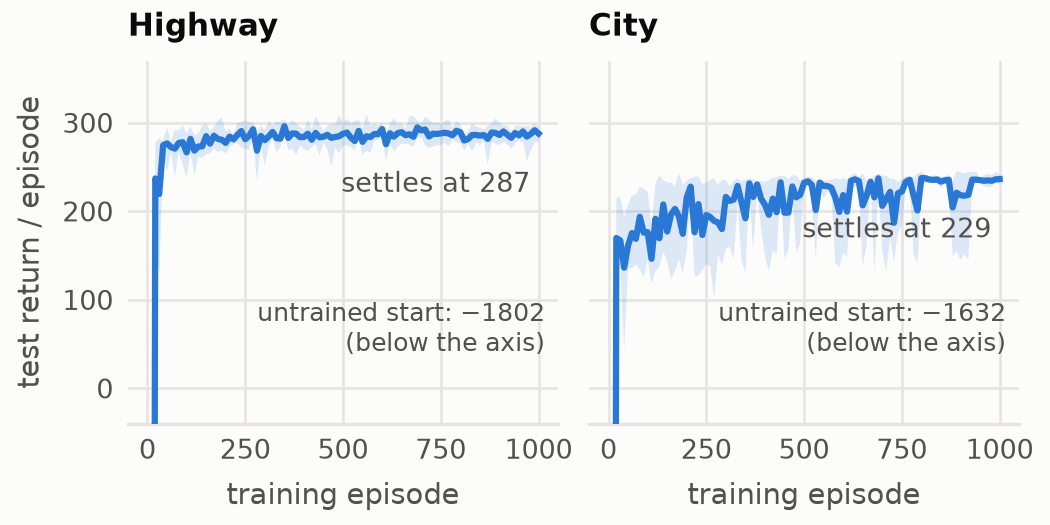
\includegraphics[width=\columnwidth]{fig_report_curve.png}
\caption{DQN learning curve: mean of 5 seeds, band = their range.}
\label{fig:curve}
\end{figure}

\begin{figure}[t]
\centering
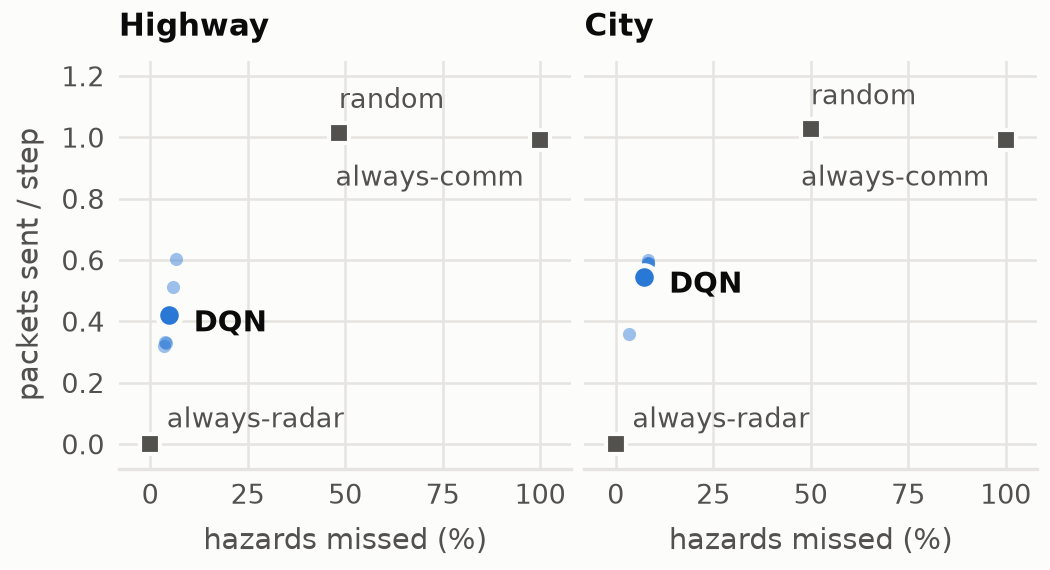
\includegraphics[width=\columnwidth]{fig_report_tradeoff.png}
\caption{Hazards missed vs.\ data sent on the 200 test drives. Top-left is
better. Small dots: the 5 DQN seeds.}
\label{fig:trade}
\end{figure}

\begin{table}[t]
\caption{Test results: 200 identical drives per policy}
\label{tab:res}
\centering\footnotesize
\setlength{\tabcolsep}{3pt}
\begin{tabular}{lrrrrr}
\toprule
Policy & Return & Missed & Sent & Urgent & Urgent \\
 & /episode & hazards \% & /step & sent \% & wait (s) \\
\midrule
\multicolumn{6}{l}{\emph{Highway}}\\
\textbf{DQN} (5 seeds) & 279 & 4.8 & 0.42 & 99 & 0.01\\
always-radar & -2203 & 0.0 & 0.00 & 0 & --\\
always-comm & -1945 & 100.0 & 0.99 & -- & --\\
random & -712 & 48.4 & 1.01 & 100 & 0.09\\
\multicolumn{6}{l}{\emph{City}}\\
\textbf{DQN} (5 seeds) & 235 & 7.3 & 0.55 & 100 & 0.02\\
always-radar & -1314 & 0.0 & 0.00 & 0 & --\\
always-comm & -2069 & 100.0 & 0.99 & -- & --\\
random & -807 & 50.1 & 1.03 & 100 & 0.09\\
\bottomrule
\end{tabular}
\end{table}


Fig.~\ref{fig:curve} shows the DQN settling after about \settle\ episodes. Table~\ref{tab:res}
and Fig.~\ref{fig:trade} show the trade-off every fixed rule gets wrong.
Always-radar misses nothing but sends nothing, so no status message and no
warning ever leaves the car. Always-communicate sends everything but misses
every hazard; random does both badly. The DQN catches \hwcatch\,\% (highway)
and \citycatch\,\% (city) of hazards, delivers \hwurg\,\% / \cityurg\,\% of urgent
warnings within \hwwait\,s / \citywait\,s on average (the 3GPP limit is
0.1\,s), and still sends \hwtput\,/\,\citytput\ packets per step. It learned
\emph{when} to look (policy tables in \texttt{runs/}): with all three conditions
good it communicates; with any condition bad and only routine traffic waiting
it uses the radar; when an urgent warning waits it mostly sends it first,
except in the worst conditions. Overall it spends \hwradar\,\% / \cityradar\,\%
of slots on radar.

\textbf{Limits.} Radar is assumed perfect and cannot see behind objects in
reality; the risk values are near-miss rates scaled from~\cite{hieu2020irdrc},
not crash data; conditions are redrawn independently every step. In both
scenarios the seeds split between two near-equal policies, sending routine
traffic or holding it back (the spread of small dots in Fig.~\ref{fig:trade});
in the city this widens the band in Fig.~\ref{fig:curve}.

\bibliographystyle{IEEEtran}
\bibliography{refs}

\end{document}
